\documentclass[conference]{IEEEtran}
% \IEEEoverridecommandlockouts
% The preceding line is only needed to identify funding in the first footnote. If that is unneeded, please comment it out.
\usepackage{cite}
\usepackage{amsmath,amssymb,amsfonts}
\usepackage{algorithmic}
\usepackage{graphicx}
\usepackage{textcomp}
\usepackage{xcolor}

\def\BibTeX{{\rm B\kern-.05em{\sc i\kern-.025em b}\kern-.08em
    T\kern-.1667em\lower.7ex\hbox{E}\kern-.125emX}}

\graphicspath{{figures/}}

\begin{document}

\title{Support Edge Based Classifiers Review}

\author{\IEEEauthorblockN{Eduardo Henrique Basilio de Carvalho}
\IEEEauthorblockA{\textit{Departamento de Engenharia Eletrônica} \\
\textit{Universidade Federal de Minas Gerais}\\
Belo Horizonte, Brasil \\
eduardohbc@ufmg.br}
}

\maketitle

\begin{abstract}
This paper reviews the theoretical foundations of Support Edge-based classifiers, a family of graph-based machine learning algorithms leveraging Gabriel Graphs for decision boundaries. We evaluate their implementation in a modern C++20 framework, focusing on computational efficiency and scalability. Potential algorithmic improvements are explored, including structural optimizations and hardware-aware modifications. Additionally, we compare high-level synthesis (HLS) implementations for embedded platforms against traditional hardware description language (HDL) approaches, assessing their viability for edge computing applications. The study aims to bridge gaps in existing methodologies while providing reproducible code and evaluation pipelines.
\end{abstract}

\begin{IEEEkeywords}
Classification, Machine Learning, Nearest Neighbor, Gabriel Graph, Support Edge
\end{IEEEkeywords}

\section{Introduction}
Support Edge-based classifiers, such as CLAS and RCHIP-CLAS, utilize geometric representations like Gabriel Graphs to define large-margin decision boundaries \cite{torres2016}. Prior work by Souza et al. \cite{souza2019} and Arias-Garcia et al. \cite{arias2021,arias2024} has demonstrated their efficacy in embedded systems, yet challenges persist in scalability and hardware optimization. Existing implementations often rely on computationally expensive adjacency matrices and may overlook optimizations in the search for inter-class edges. This review addresses these limitations by proposing algorithmic refinements and evaluating modern hardware synthesis tools. By integrating software optimizations with high-level synthesis workflows, we aim to enhance the feasibility of these classifiers for real-time edge applications.

\section{Theoretical Background}
\subsection{Gabriel Graph (GG)}
The Gabriel Graph (GG) is a type of planar graph derived from a set of points in a Euclidean space. For a dataset \(\mathcal{D} = \{(\mathbf{x}_i, y_i)\}\), where \(\mathbf{x}_i \in \mathbb{R}^n\) and \(y_i \in \{+1, -1\}\), the GG is constructed such that two vertices \(\mathbf{x}_i\) and \(\mathbf{x}_j\) are connected by an edge if and only if no other vertex \(\mathbf{x}_z\) lies within the hypersphere with \(\mathbf{x}_i\) and \(\mathbf{x}_j\) as its diameter. Formally, this condition is expressed as:
\[
\delta^2(\mathbf{x}_i, \mathbf{x}_j) \leq \delta^2(\mathbf{x}_i, \mathbf{x}_z) + \delta^2(\mathbf{x}_j, \mathbf{x}_z), \quad \forall \mathbf{x}_z \in \mathcal{D}, \mathbf{x}_z \neq \mathbf{x}_i, \mathbf{x}_j,
\]
where \(\delta(\cdot)\) denotes the Euclidean distance operator. The GG inherently captures the structural relationships between data points and is computationally efficient when built using Delaunay triangulation, reducing its complexity to \(O(n \log n)\) in planar cases \cite{arias2021, torres2015b}.

\subsection{Support Edges (SE)}
Support Edges (SE) are a subset of edges in the GG that connect vertices from opposing classes (\(y_i \neq y_j\)). These edges lie on the separation margin between classes and are analogous to Support Vectors in SVMs. The midpoint \(\mathbf{p}_l = \frac{\mathbf{x}_i + \mathbf{x}_j}{2}\) of each SE defines a local hyperplane \(H_l\) orthogonal to the edge, serving as a maximal margin classifier for the pair \((\mathbf{x}_i, \mathbf{x}_j)\). The SE set \(\mathcal{AS}\) is unique to the dataset and forms the basis for constructing large-margin classifiers \cite{torres2016, torres2015b}.

\subsection{Data Filtering}
To handle noisy or overlapping data, a quality measure \(q(\mathbf{x}_i)\) filters vertices based on their connectivity in the GG. For a vertex \(\mathbf{x}_i\), let \(\mathcal{A}(\mathbf{x}_i)\) denote its degree (number of connected edges) and \(\hat{\mathcal{A}}(\mathbf{x}_i)\) the number of edges connecting \(\mathbf{x}_i\) to vertices of the same class. The quality measure is defined as:
\[
q(\mathbf{x}_i) = \frac{\hat{\mathcal{A}}(\mathbf{x}_i)}{\mathcal{A}(\mathbf{x}_i)}.
\]
Vertices with \(q(\mathbf{x}_i) < t^\pm\) (class-specific thresholds) are removed. Thresholds \(t^+\) and \(t^-\) are computed as the average of \(q(\mathbf{x}_i)\) values within each class:
\[
t^+ = \frac{1}{|\Omega^+|}\sum_{q(\mathbf{x}_i) \in \Omega^+} q(\mathbf{x}_i), \quad t^- = \frac{1}{|\Omega^-|}\sum_{q(\mathbf{x}_i) \in \Omega^-} q(\mathbf{x}_i),
\]
where \(\Omega^\pm\) are the quality measures grouped by class. This step ensures robust SE detection \cite{arias2021, torres2016}.

\subsection{CHIP-CLAS}
CHIP-CLAS is a large-margin classifier that combines hyperplanes derived from SEs via a Hierarchical Mixture of Experts (HME). Each hyperplane \(H_l\) is defined by:
\[
H_l(\mathbf{x}) = \text{sign}(\mathbf{x}^T \mathbf{w}_l - b_l),
\]
where \(\mathbf{w}_l = \mathbf{x}_i - \mathbf{x}_j\) (normal vector) and \(b_l = \frac{1}{2}(\mathbf{x}_i + \mathbf{x}_j)^T \mathbf{w}_l\) (bias term). The final classification aggregates weighted outputs from all hyperplanes:
\[
f(\mathbf{x}) = \text{sign}\left(\sum_{l=1}^m h_l(\mathbf{x}) c_l(\mathbf{x})\right),
\]
with weights \(c_l(\mathbf{x})\) computed as:
\[
c_l(\mathbf{x}) = \exp\left(-\frac{\max(\delta(\mathbf{x}, \mathbf{p}_k))^2}{\delta(\mathbf{x}, \mathbf{p}_l)}\right), \quad \sum_{l=1}^m c_l(\mathbf{x}) = 1.
\]
This method optimizes margin maximization and training error minimization without user-defined parameters \cite{torres2015, torres2015b}.

\subsection{RCHIP-CLAS}
RCHIP-CLAS is a reduced-complexity variant of CHIP-CLAS. Instead of combining all hyperplanes, it selects the hyperplane closest to the test sample \(\mathbf{x}\) using:
\[
\arg\min_l \delta(\mathbf{x}, \mathbf{p}_l), \quad l = 1, \ldots, m,
\]
where \(\mathbf{p}_l\) is the midpoint of the \(l\)-th SE. The classification rule simplifies to:
\[
f(\mathbf{x}) = \begin{cases} 
+1 & \text{if } H_l(\mathbf{x}) > 0, \\
-1 & \text{otherwise}.
\end{cases}
\]
This approach reduces computational overhead while maintaining accuracy \cite{arias2021}.

\subsection{NN-CLAS}
NN-CLAS further simplifies classification by applying a nearest-neighbor rule on the SE vertices. For a test sample \(\mathbf{x}\), its class is assigned as the label of the closest SE vertex:
\[
\hat{y} = y_{\arg\min_i \delta(\mathbf{x}, \mathbf{x}_i)}, \quad \mathbf{x}_i \in \mathcal{AS}.
\]
This method eliminates hyperplane computations and is equivalent to \(k\)-NN (\(k=1\)) restricted to margin points, making it highly efficient for hardware implementation \cite{souza2019, arias2021}.

\section{Possible Improvements}
Two key algorithmic improvements are proposed. First, replacing adjacency matrices with adjacency lists reduces memory complexity from $O(n^2)$ to $O(n + \left|E|\right)$, where $|E|$ is the number of edges in the Gabriel Graph. This is particularly advantageous for sparse datasets. Second, post-filtering steps can be optimized by computing edges exclusively between points of opposing classes, eliminating redundant intra-class calculations. This approach leverages class label metadata early in the pipeline, reducing computational overhead during graph construction.

\section{Methodology}
The implementation, available at \texttt{https://github.com/eduardo-ufmg/CLAS}, employs C++20 for classifier development. Synthetic datasets—generated via Python's \texttt{sklearn}—are used to evaluate decision boundaries under varying geometric complexities. Python scripts automate performance benchmarking, including accuracy and latency measurements. For hardware evaluation, Vitis HLS synthesizes the classifiers for two platforms: the Alveo U55C (data center-grade FPGA) and Zedboard (embedded FPGA). The HLS workflows are compared against hand-optimized Verilog/VHDL implementations to assess trade-offs in resource utilization and throughput.

\section{Results}
% Results section figures
\begin{figure}[htbp]
\centering
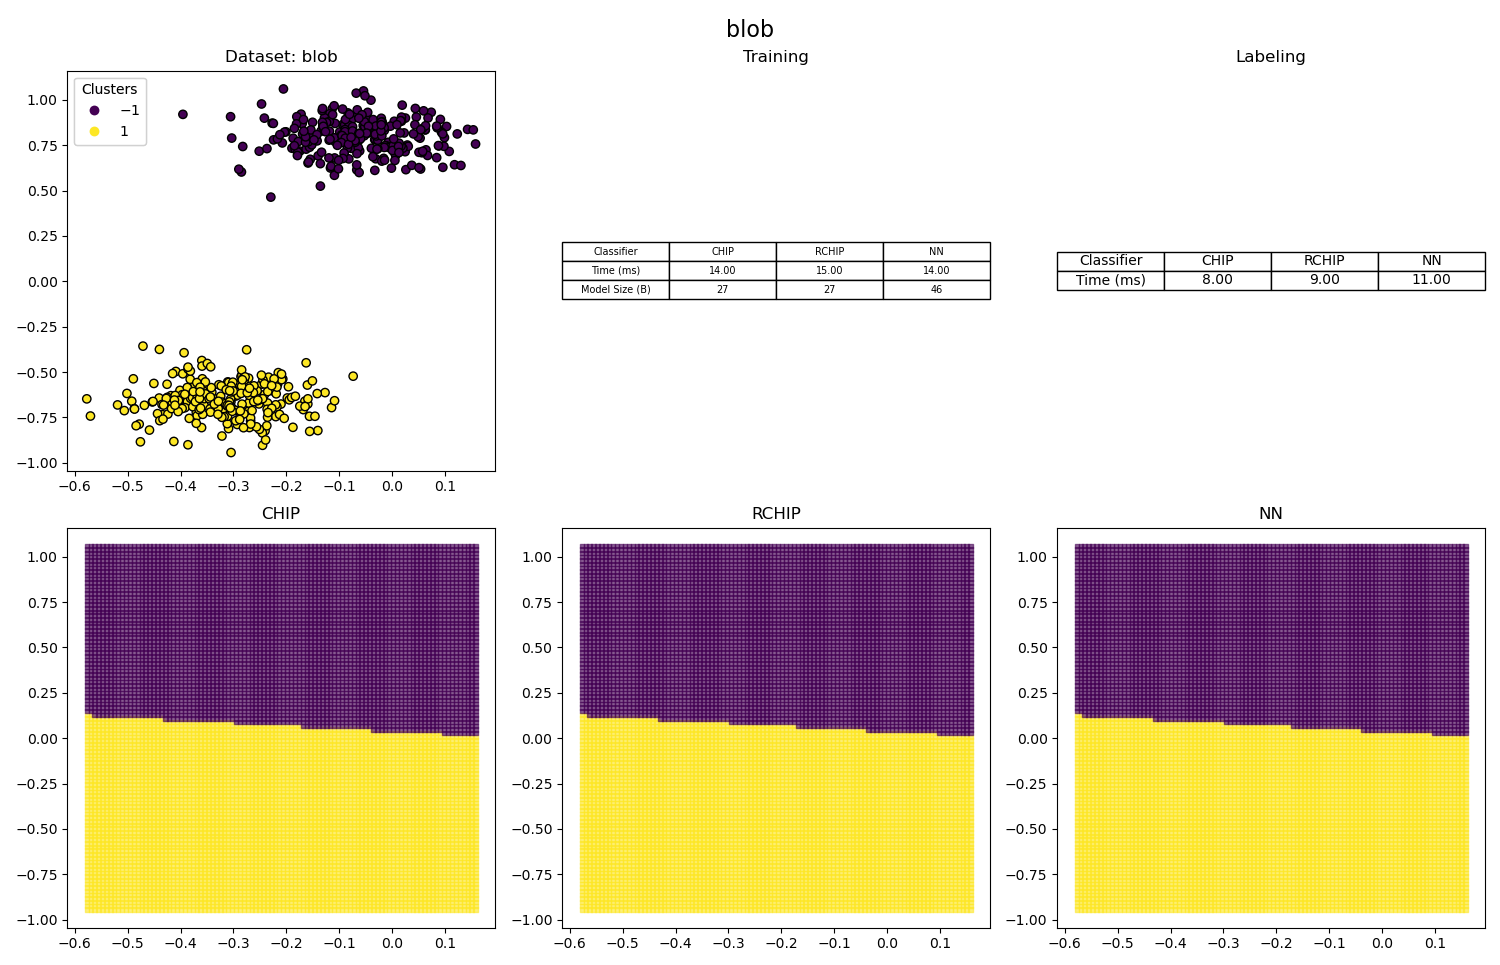
\includegraphics[width=1.00\linewidth]{blob_good.png}
\caption{Good classification results on linearly separable data.}
\label{fig:blob_good}
\end{figure}

\begin{figure}[htbp]
\centering
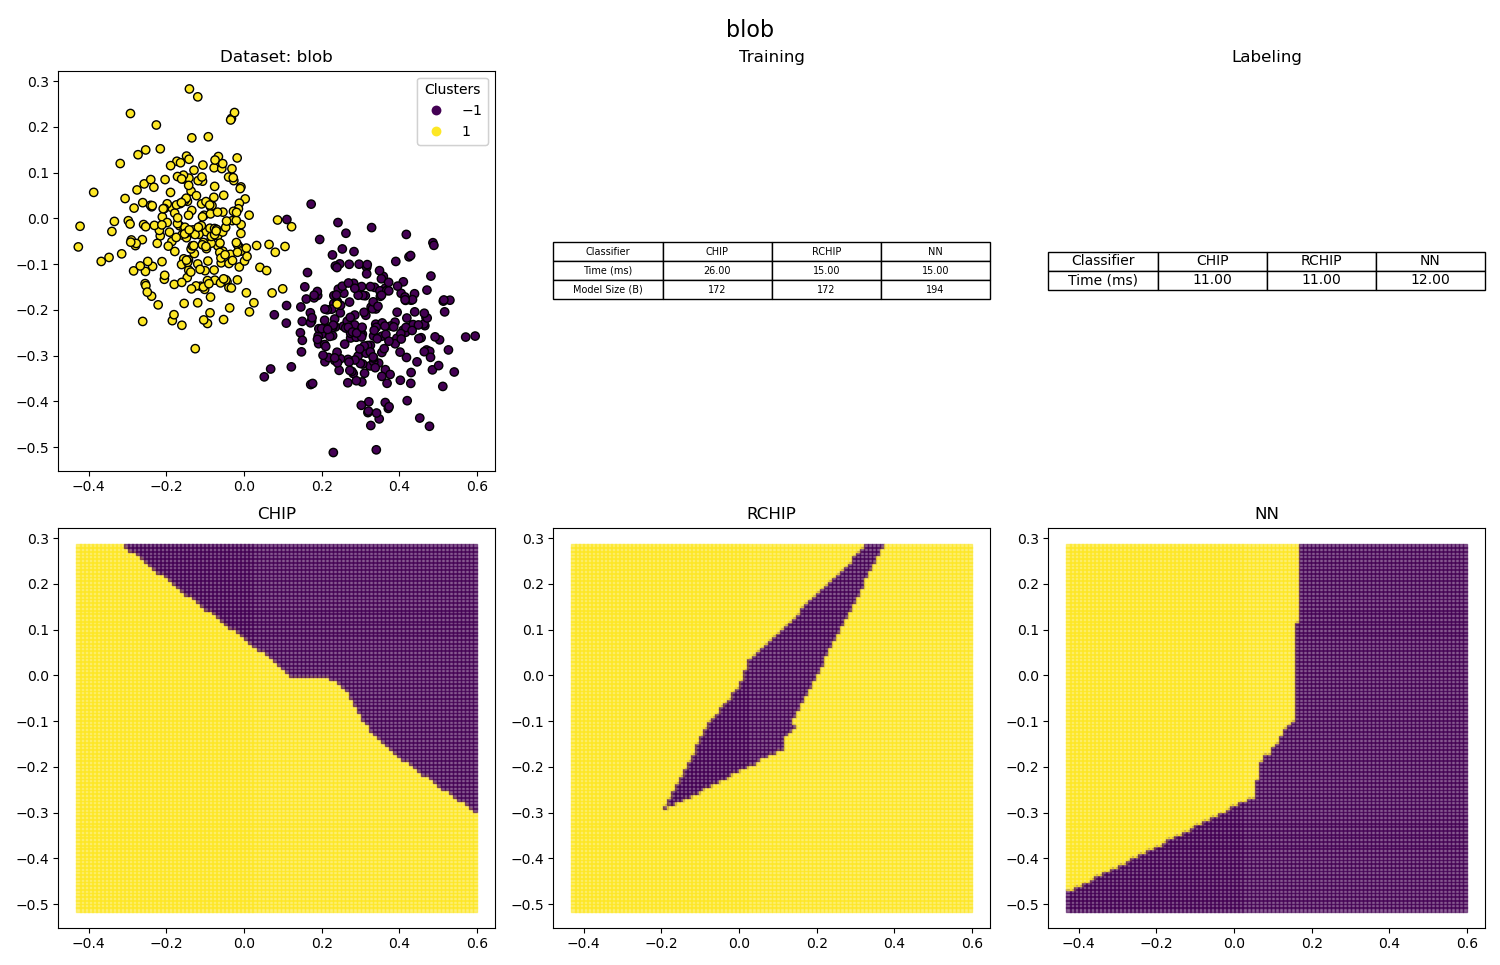
\includegraphics[width=1.00\linewidth]{blob_bad.png}
\caption{Bad classification results on linearly separable data.}
\label{fig:blob_bad}
\end{figure}

\begin{figure}[htbp]
\centering
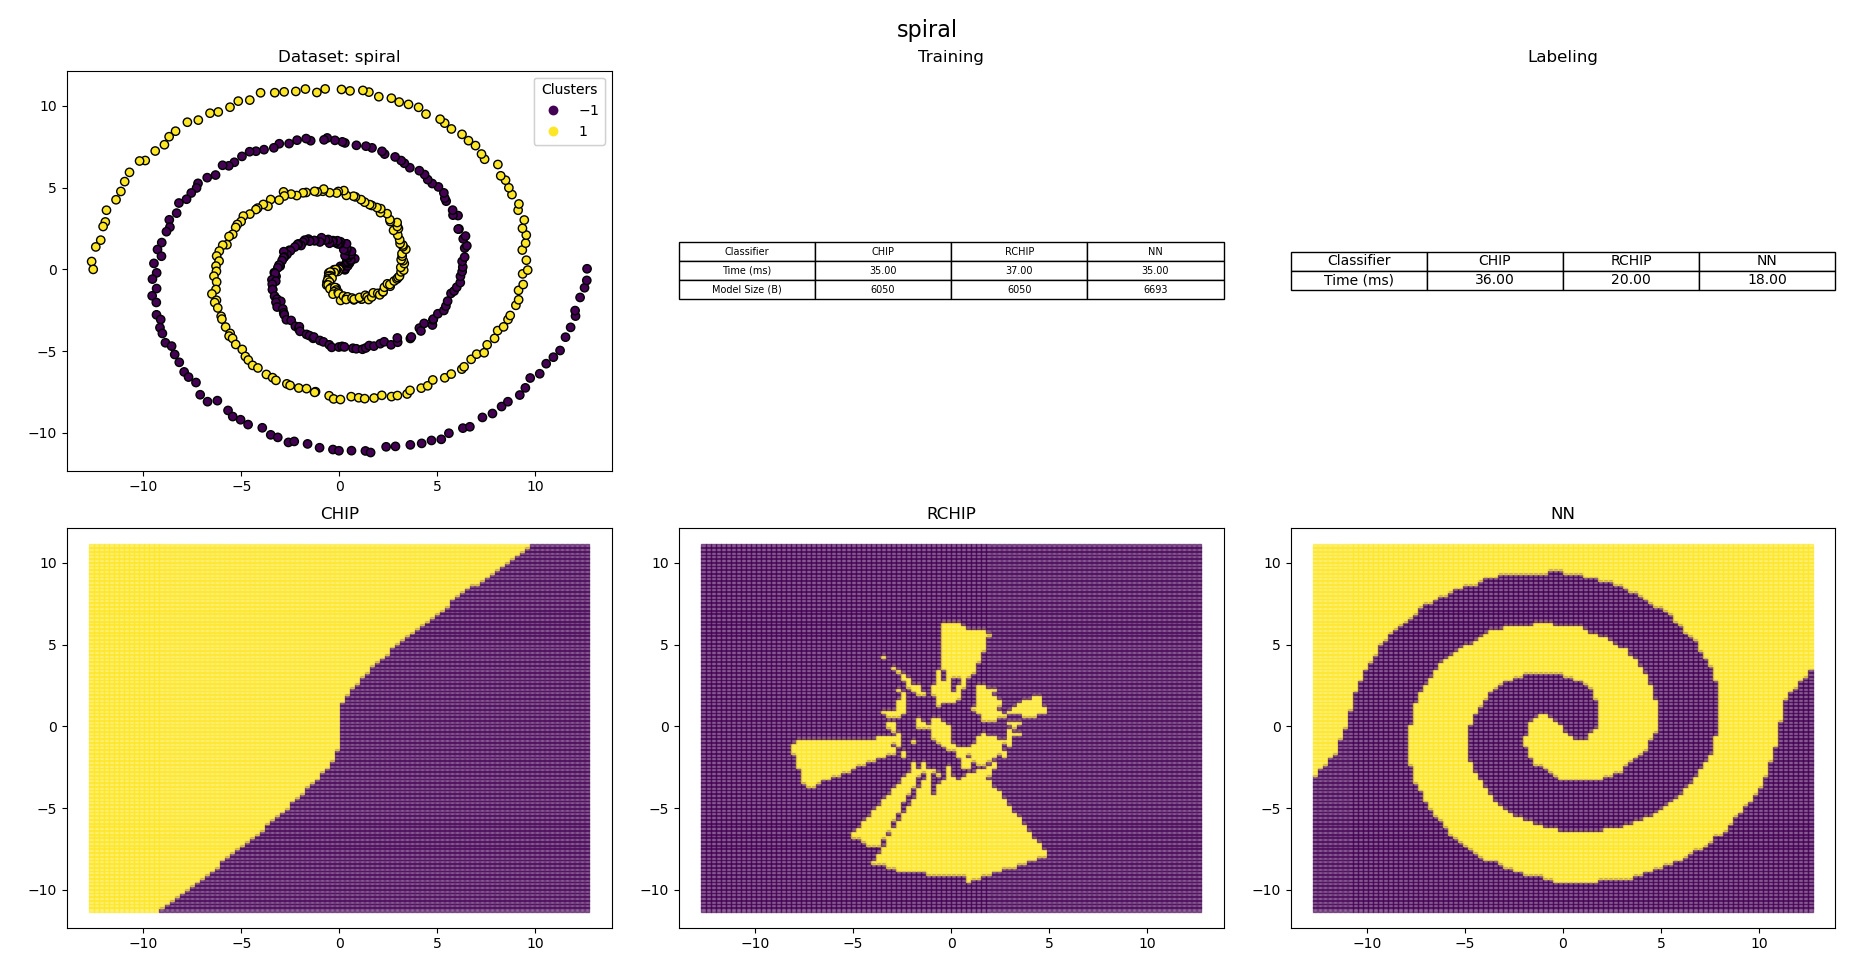
\includegraphics[width=1.00\linewidth]{spiral.png}
\caption{Classification results on spiral dataset.}
\label{fig:spiral}
\end{figure}

\begin{figure}[htbp]
\centering
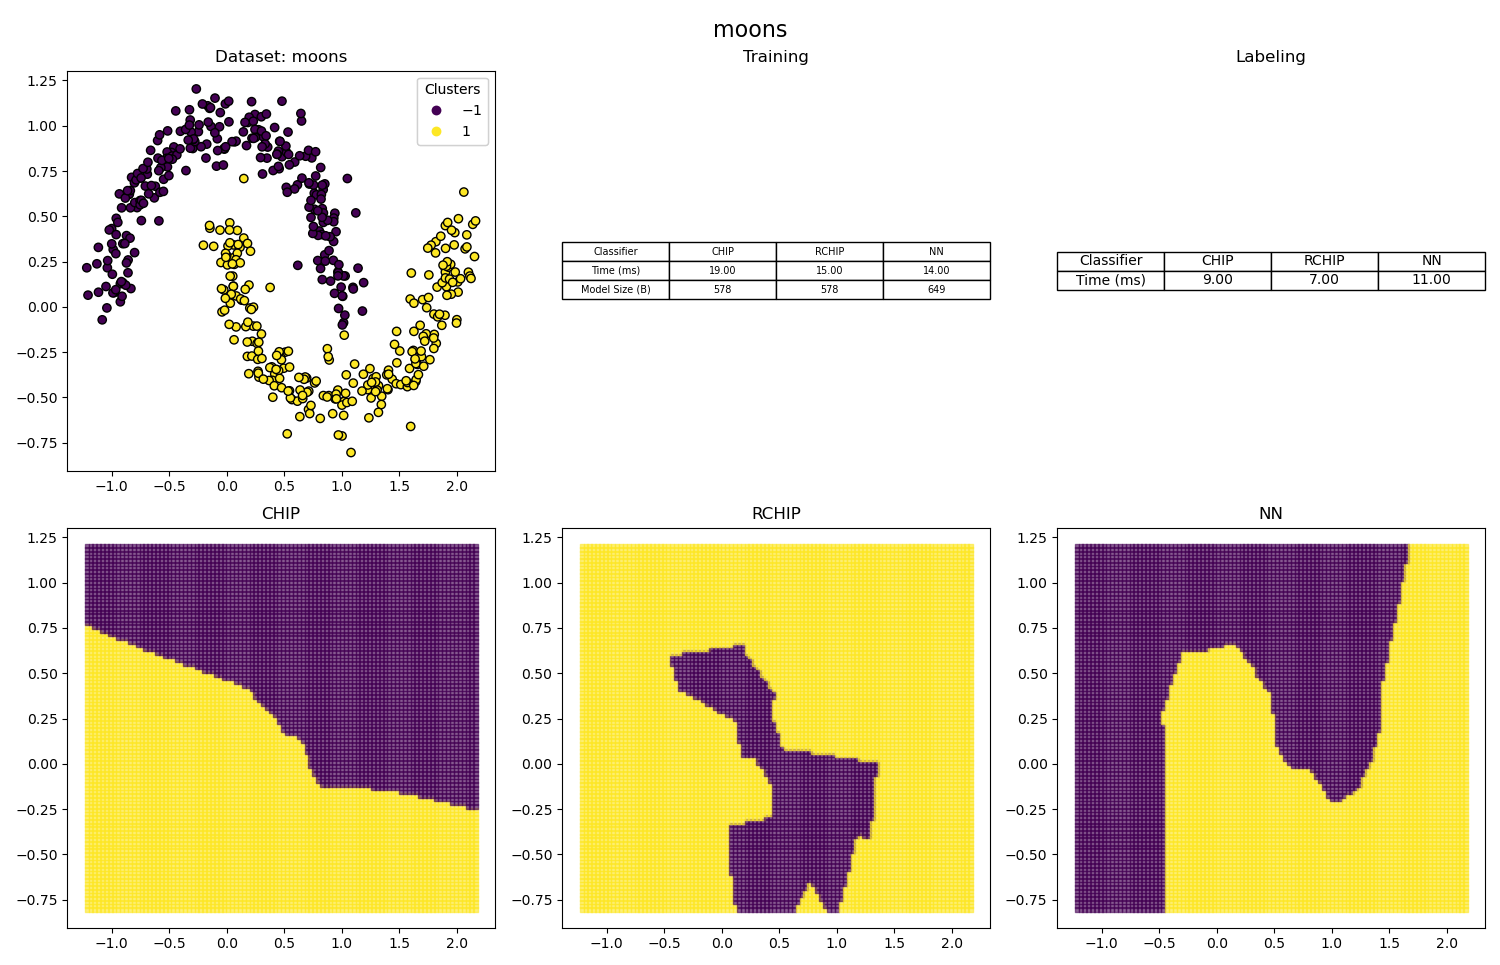
\includegraphics[width=1.00\linewidth]{moons.png}
\caption{Classification results on moons dataset.}
\label{fig:moons}
\end{figure}

\begin{figure}[htbp]
\centering
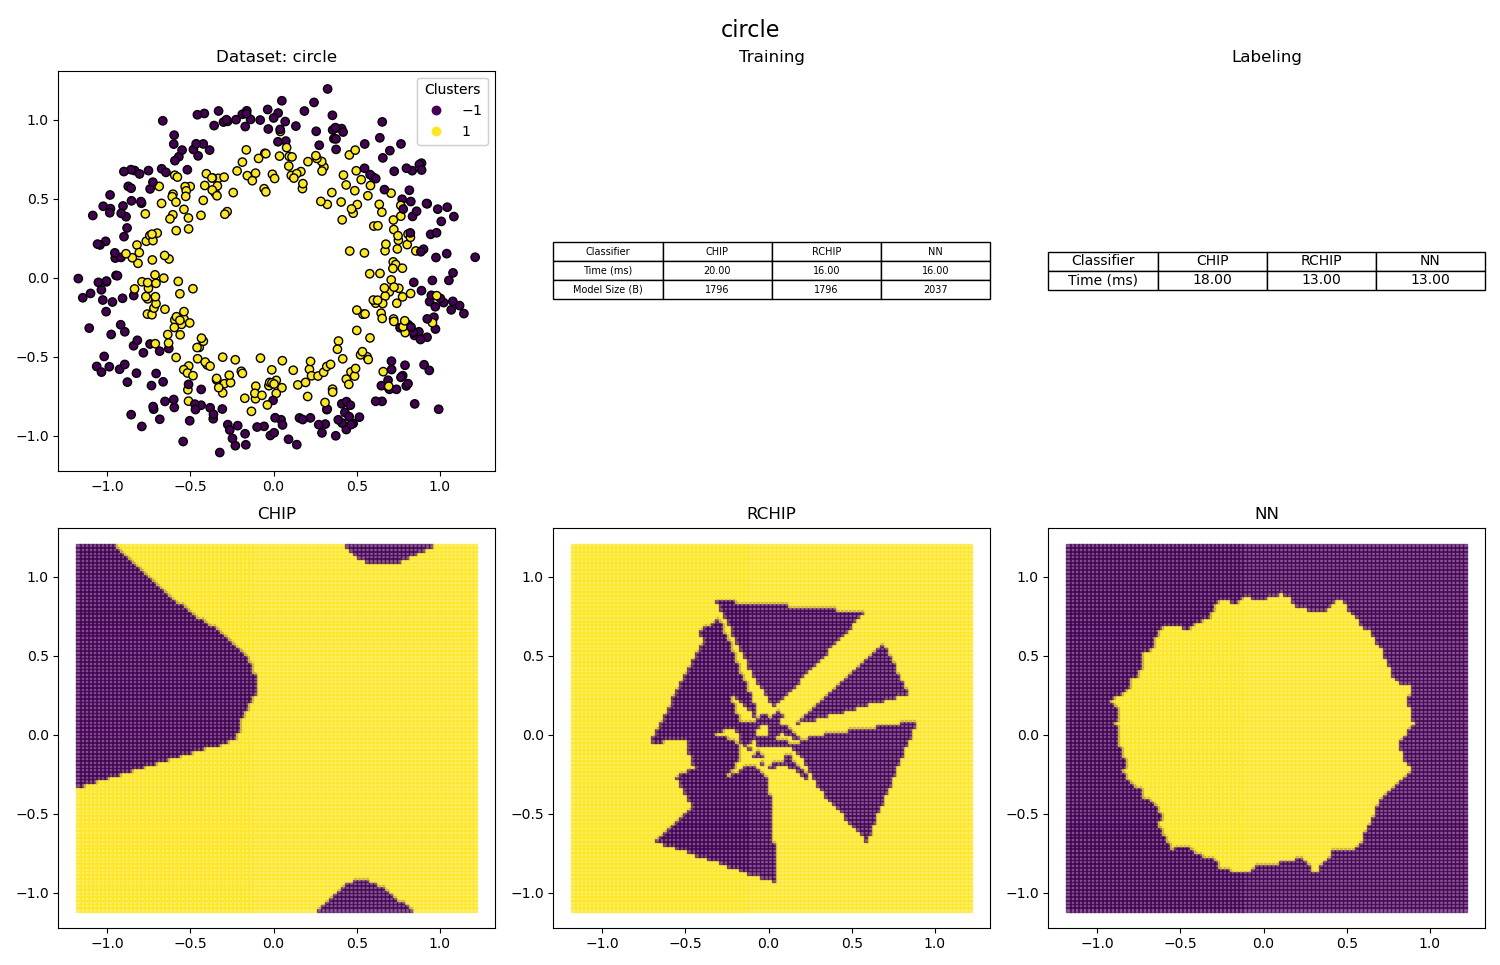
\includegraphics[width=1.00\linewidth]{circles.png}
\caption{Classification results on concentric circles dataset.}
\label{fig:circles}
\end{figure}

\begin{figure}[htbp]
\centering
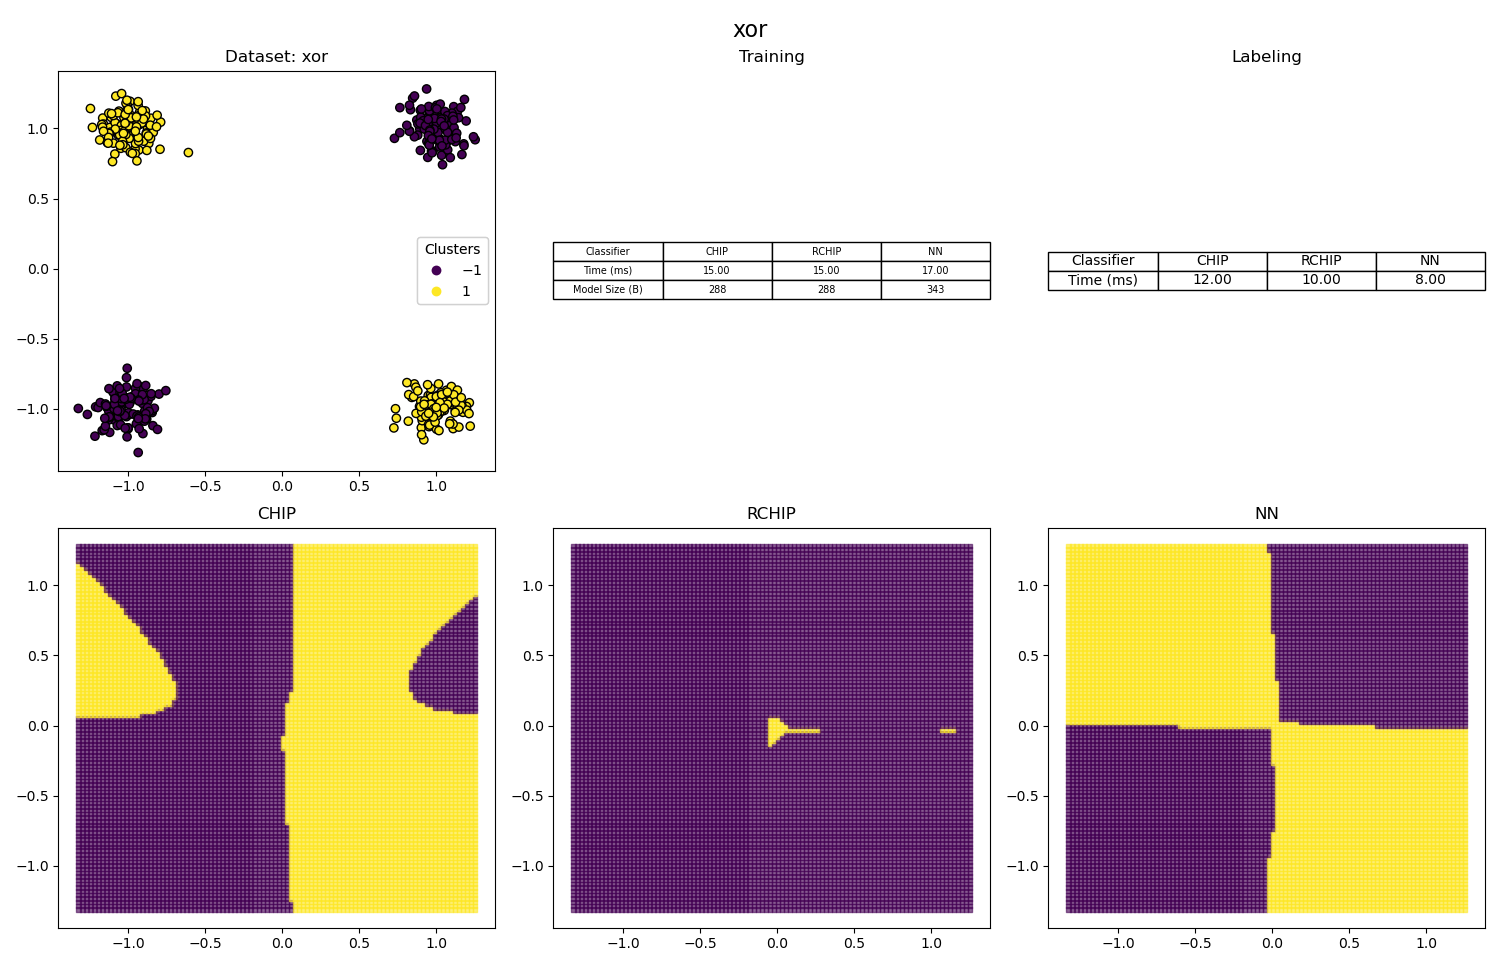
\includegraphics[width=1.00\linewidth]{xor.png}
\caption{Classification results on XOR dataset.}
\label{fig:xor}
\end{figure}

\begin{thebibliography}{00}
\bibitem{torres2016} L. C. B. Torres, "Classificador por arestas de suporte (CLAS): métodos de aprendizado baseados em Grafos de Gabriel," Manuscript, 2016.
\bibitem{souza2019} A. C. Souza, C. Leite Castro, J. A. Garcia, L. C. B. Torres, L. J. Acevedo Jaimes and B. R. A. Jaimes, "Improving the Efficiency of Gabriel Graph-based Classifiers for Hardware-optimized Implementations," 2019 XXII Symposium on Image, Signal Processing and Artificial Vision (STSIVA), Bucaramanga, Colombia, 2019.
\bibitem{arias2021} J. Arias-Garcia et al., "Enhancing Performance of Gabriel Graph-Based Classifiers by a Hardware Co-Processor for Embedded System Applications," in IEEE Transactions on Industrial Informatics, vol. 17, no. 2, Feb. 2021.
\bibitem{arias2024} J. Arias-Garcia et al., "Improved Design for Hardware Implementation of Graph-Based Large Margin Classifiers for Embedded Edge Computing," in IEEE Transactions on Neural Networks and Learning Systems, vol. 35, no. 1, Jan. 2024.
\bibitem{torres2015} L. C. B. Torres, C. L. Castro and A. P. Braga, "A parameterless mixture model for large margin classification," 2015 International Joint Conference on Neural Networks (IJCNN), Killarney, Ireland, 2015.
\bibitem{torres2021} L. C. B. Torres, C. L. Castro, F. Coelho and A. P. Braga, "Large Margin Gaussian Mixture Classifier With a Gabriel Graph Geometric Representation of Data Set Structure," in IEEE Transactions on Neural Networks and Learning Systems, vol. 32, no. 3, March 2021.
\bibitem{torres2015b} L. C. B. Torres, C. L. Castro, F. Coelho, F. Sill Torres and A. P. Braga, "Distance-based large margin classifier suitable for integrated circuit implementation," Manuscript, 2015.
\end{thebibliography}

\end{document}
